\documentclass[utf8x,xcolor=pdftex,dvipsnames,table]{beamer}
\usetheme{Malmoe}  % Now it's a beamer presentation with the lisa theme!
\setbeamertemplate{footline}[page number]
\usecolortheme{beaver}
\usepackage[T1]{fontenc}
\usepackage{amsmath}
\usepackage[utf8x]{inputenc}
\usepackage{listings}

\newcommand{\superscript}[1]{\ensuremath{^{\textrm{#1}}}}

\mode<presentation>

\title{Debugging}

\author{%
\footnotesize
Frédéric Bastien \newline
\newline
\newline
Institut des algorithmes d'apprentissage de Montréal \newline
Montreal Institute for Learning Algorithms \newline
Université de Montréal
}

\date{August 10th, Deep Learning Summer School 2015, Montréal}

\setbeamertemplate{navigation symbols}{}
\begin{document}

\begin{frame}[plain]
 \titlepage
 \vspace{-2em}
 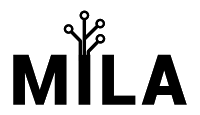
\includegraphics[width=.8in]{mila.png}
 \hfill
 
\includegraphics[width=.8in]{UdeM_logo}
\end{frame}

\section{Introduction}
\begin{frame}{Slides and Exercices}
  \url{http://github.com/mila-udem/summerschool2015/debug}
\end{frame}

\section{Debugging}
\begin{frame}
  \tableofcontents[currentsection]
\end{frame}


\subsection{Error message}
\begin{frame}[fragile]
  \frametitle{Error message: code}
\lstset{language=Python,
        commentstyle=\itshape\color{blue},
        stringstyle=\color{violet},
        }
\begin{lstlisting}
import numpy as np
import theano
import theano.tensor as T
x = T.vector()
y = T.vector()
z = x + x
z = z * y
f = theano.function([x, y], z)
f(np.ones((2,)), np.ones((3,)))
\end{lstlisting}
\end{frame}

\begin{frame}[fragile]
  \frametitle{Error message: 1st part}

\lstset{language=Python,
        commentstyle=\itshape\color{blue},
        stringstyle=\color{violet},
        basicstyle=\scriptsize
        }
\begin{lstlisting}
Traceback (most recent call last):
[...]
ValueError: Input dimension mis-match.
    (input[0].shape[0] = 2, input[1].shape[0] = 3)
Apply node that caused the error:
     Elemwise{Composite{((i0 + i0) * i1)}}(
         <TensorType(float64, vector)>,
         <TensorType(float64, vector)>)
Toposort index: 0
Inputs types: [TensorType(float64, vector),
               TensorType(float64, vector)]
Inputs shapes: [(2,), (3,)]
Inputs strides: [(8,), (8,)]
Inputs values: [array([ 1.,  1.]), array([ 1.,  1.,  1.])]
Outputs clients: [['output']]
\end{lstlisting}
\end{frame}

\begin{frame}[fragile]
  \frametitle{Error message: 2st part}
HINT: Re-running with most Theano optimization
disabled could give you a back-traces when this
node was created. This can be done with by setting
the Theano flags ``optimizer=fast\_compile''. If that does not
work, Theano optimizations can be disabled with
``optimizer=None''.\newline
HINT: Use the Theano flag ``exception\_verbosity=high''
for a debugprint of this apply node.
\end{frame}


\begin{frame}[fragile]
  \frametitle{Error message: Traceback}

\lstset{language=Python,
        commentstyle=\itshape\color{blue},
        stringstyle=\color{violet},
        basicstyle=\footnotesize,
        xleftmargin=-1em
        }
\begin{lstlisting}
Traceback (most recent call last):
  File "test.py", line 9, in <module>
    f(np.ones((2,)), np.ones((3,)))
  File "/u/bastienf/repos/theano/compile/function_module.py",
       line 589, in __call__
    self.fn.thunks[self.fn.position_of_error])
  File "/u/bastienf/repos/theano/compile/function_module.py",
       line 579, in __call__
    outputs = self.fn()
\end{lstlisting}
\end{frame}


\begin{frame}[fragile]
  \frametitle{Error message: optimizer=fast\_compile}

\lstset{language=Python,
        commentstyle=\itshape\color{blue},
        stringstyle=\color{violet},
        }
\begin{lstlisting}
Backtrace when the node is created:
  File "test.py", line 7, in <module>
    z = z * y

\end{lstlisting}
\end{frame}

\subsection{DebugMode}
\begin{frame}[fragile]
  \frametitle{DebugMode}
    Checks and double-checks everything, extremely slow
\begin{itemize}
\item Compare Python, C and GPU implementations.
\item Compare before and after each optimization.
\item By default, raise an error on NaN.
\item Sensitive: so frequently reported errors are ok.
\end{itemize}
\end{frame}

\subsection{Breakpoint}
\begin{frame}[fragile]
  \frametitle{Breakpoint Op} Identity-like op with the side effect of
  enforcing a conditional breakpoint, inside a theano function, based
  on a symbolic scalar condition.
\end{frame}

\begin{frame}[fragile]
  \frametitle{Breakpoint Op: optimization}
  Theano optimization don't know it.
\begin{itemize}
  \item Could Slow down computation, but not too much.
  \item Could disable stability optimization
  \item It is moved to the GPU (it do not force transfer)
\end{itemize}
\end{frame}

\begin{frame}[fragile]
  \frametitle{Breakpoint Op: example}
\lstset{language=Python,
        commentstyle=\itshape\color{blue},
        stringstyle=\color{violet},
        basicstyle=\footnotesize,
        xleftmargin=-1em
        }
\begin{lstlisting}
import theano
import theano.tensor as T
from theano.tests.breakpoint import PdbBreakpoint
input, target = T.fvectors('xy')

mse = (input - target) ** 2

# Conditional breakpoint to be activated if the total MSE is higher
# than 100. The breakpoint will monitor the inputs, targets as well
# as the individual error values
breakpointOp = PdbBreakpoint(``MSE too high'')
condition = T.gt(mse.sum(), 100)
mse, monitored_input, monitored_target = breakpointOp(
    condition, mse, input, target)
\end{lstlisting}
\end{frame}

\begin{frame}[fragile]
  \frametitle{Breakpoint Op: example}
\lstset{language=Python,
        commentstyle=\itshape\color{blue},
        stringstyle=\color{violet},
        basicstyle=\footnotesize,
        xleftmargin=-1em
        }
\begin{lstlisting}
# Compile the theano function
fct = theano.function([input, target], mse)

# Use the function
print fct([10, 0], [10, 5]) # Will NOT activate the breakpoint
print fct([0, 0], [10, 5]) # Will activate the breakpoint
\end{lstlisting}

\end{frame}

\subsection{PrintOp}
\begin{frame}
  \frametitle{PrintOp}
\end{frame}


\subsection{Nan}
\begin{frame}
  \frametitle{NanGuardMode}
\end{frame}

\subsection{Test Value}
\begin{frame}
  \frametitle{test value}
\end{frame}

\subsection{Others}
\begin{frame}
  \frametitle{Others}
  \begin{itemize}
  \item theano.tensor.opt.AssertOp
  \item theano.printig.{debugprint,pydotprint}


  \item Flag: profile=True
  \item Flag: exception\_verbosity=True (ex: for Memory Error)
  \item Flag: on\_opt\_err=True
  \item Flag: optimizer\_verbose=True
  \item Flag: warn\_float64=True
  \end{itemize}
\end{frame}

\section{Python Debugger}
\begin{frame}
  \begin{itemize}
  \item pdb, is the python debugger
  \end{itemize}

  Can be combined with those Theano flags to disable Theano c code:
  \begin{itemize}
    \item mode=FAST\_COMPILE \# Disable most of Theano opt + c code.
    \item linker=py \# Disable Theano c code.
  \end{itemize}
\end{frame}

\begin{frame}{Connection instructions}
\begin{itemize}
\item Navigate to \url{nvlabs.qwiklab.com}
\item Login or create a new account
\item Select the ``Instructor-Led Hands-on Labs'' class
\item Find the lab called ``Theano'' and click Start
\item After a short wait, lab instance connection information will be shown
\item Please ask Lab Assistants for help!
\end{itemize}
\end{frame}

\begin{frame}{Questions, Acknowledgments}
\Huge
\begin{center}
Questions?\newline
Acknowledgments
\end{center}
\normalsize
\begin{itemize}
\item All people working or having worked at the LISA lab/MILA institute
\item All Theano users/contributors
\item Compute Canada, RQCHP, NSERC, and Canada Research Chairs for providing funds or access to compute resources.
\end{itemize}

\end{frame}


\end{document}
